\section{Motor-Treiber (Specht)}

Wesentlich für den Einstieg in die Motor-Treiber-Programmierung waren die verwendeten Hardware-Komponenten. Folgende Teile wurden verwendet:

\begin{itemize}
    \item 2x Pololu G2 High-Power Motor Driver 24v13 (MD31C)
    \item 2x MFA/Como Drills 919D501
\end{itemize}

Im ersten Ansatz wurde der Versuch unternommen, den Low-Level-Treiber (LL-Treiber) direkt mit der Differenzialantriebs-Logik (Differentialantrieb) zu koppeln. Nach intensiver Recherche und ersten Programmieransätzen wurde jedoch deutlich, dass eine klare Trennung beider Ebenen unter modularen Gesichtspunkten vorzuziehen ist. Diese Trennung resultiert in einer signifikanten Steigerung sowohl der Wiederverwendbarkeit als auch der Wartbarkeit des Codes. Abhilfe schafften hierbei vor allem die Verwendung von ESP-IDF-Komponenten.\newline

Um die Ansteuerung der Motoren zu realisieren, war es von zentraler Bedeutung, die Spezifikationen der verwendeten Hardware zu berücksichtigen. Das Datenblatt der Pololu-Motor-Treiber wurde in Form einer Webseite gefunden. Die darin enthaltenen Informationen waren ausreichend, um die Logik zu implementieren. Für die verwendeten Motoren lieferte das Datenblatt insbesondere elektrische Kenngrößen, die für die Absicherung der Hardware von entscheidender Bedeutung waren. Dazu zählten maximale und nominale Ströme. Zu Beginn des Projektes konnte nur auf einen 6V-Akku zurückgegriffen werden, obwohl die Motoren bis zu 12V-Betriebsspannung zulassen. Daraufhin wurden entsprechende Widerstände auf den Treiberboards angebracht, um den maximalen Strom für 6V zu begrenzen. Des Weiteren konnte aus dem Datenblatt des Pololu-Motor-Treibers die Notwendigkeit überdimensionierter Kondensatoren abgeleitet werden, um eine gute und stabile Performance sicherzustellen. \newline

Der Fokus der Implementierung lag vorrangig auf Modularität, Erweiterbarkeit, Clean-Code und Best-Practices. Dafür wurde wenn möglich auf globale Variablen verzichtet und stattdessen auf die Verwendung von Strukturen und Funktionen in Kombination mit Pointern gesetzt.

\subsection{Low-Level Treiber}

Die Aufgabe des LL-Treibers bestand darin, genau einen Motor anzusprechen und zu steuern. Das verwendete Framework ESP-IDF bietet eine Vielzahl an API-Funktionen, die eine abstrahierte und einfache Ansteuerung der Hardware ermöglichen. Für das Erzeugen von PWM-Signalen sind vor allem zwei API's von zentraler Bedeutung:

\begin{itemize}
    \item LED Control (LEDC)
    \item Motor Control Pulse Width Modulator (MCPWM)
\end{itemize}

Wie den Namen zu entnehmen ist, ist LEDC für die einfache Ansteuerung von LEDs gedacht, während MCPWM speziell für Motoren entwickelt wurde. Der MCPWM-Generator besteht aus einer Reihe von Submodulen, wie bspw. einem Fault-Module und einem Brake-Operator. Die Pololu-Boards bieten ebenfalls einen Fault-Pin, weshalb im weiteren Projektverlauf der MCPWM-Generator verwendet wurde, um diese Funktionalität nutzen zu können. \newline

Die MCPWM-API umfasst mehrere Funktionen und Strukturen. Deswegen wurde der erste Entwurf auf Basis einer Kombination aus KI-generiertem Code und Beispielcode von Github erstellt. Die grundlegende Funktionalität konnte dadurch unkompliziert und schnell erfasst werden, wodurch Zeit gespart wurde. Nichtsdestotrotz war es notwendig, entsprechende Literatur zur API zu lesen und zu verstehen. Im Folgenden wurde der Code Stück für Stück angepasst, modularisiert und erweitert. \newline

Ein Key-Konzept entstand aus dem Gedanken, was passieren würde, wenn ein Duty-Cycle von beispielsweise 100 \% (Volllast) gesetzt wird und die Drehrichtung des Motors umgekehrt wird. Die Annahme war, dass der Motortreiber + und - umpolen würde und der Motor währenddessen solange als Generator arbeitet, bis die Richtung letztendlich umgekehrt wird. Der dabei möglicherweise auftretende Rückstrom könnte eventuell die Hardware beschädigen. Aus diesem Grund wurde sich auf eine Ramping-Strategie geeinigt, die eine sichere und kontrollierte Änderung der Drehrichtung ermöglicht. Dabei soll sichergestellt werden, dass der Duty-Cycle des PWM-Signals bzw. die Richtung für den Motor nicht abrupt geändert wird. Stattdessen wird der Duty-Cycle in konfigurierbaren Schritten dem Nullbereich angenähert. In einem sicheren Hysteresebereich wird dann die Richtung geändert und der Duty-Cycle der neuen gewünschten Geschwindigkeit angepasst. \newline

Ein weiterer wichtiger Baustein sollte das automatisierte Erkennen von Fehlern der Motoren sein. In solch einem Fall sollte der Motor sofort gestoppt werden und eine Signalleuchte angehen. Ein einfacher Testaufbau bestehend aus Pull-up Widerständen und einer LED sollte die grundlegende Funktionalität des Fault-Pins sicherstellen.

\begin{figure}[h]
    \centering
    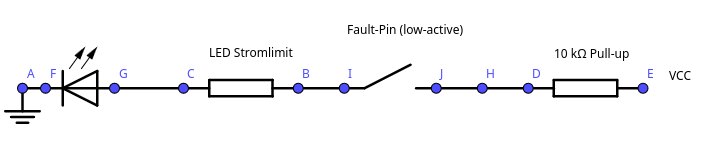
\includegraphics[width=\textwidth]{images/motor_driver_fault_pin.png}
    \caption{Testaufbau des Fault-Pins des Pololu-Motor-Treibers}
    \label{fig:motor_driver_fault_pin}
\end{figure}

Der Fault-Pin ist laut Datenblatt ein Open-Drain-Ausgang, der bei einem Fehler auf Low gezogen wird. Im Testaufbau wurde ein Pull-Up-Widerstand von 10 k$\Omega$ verwendet, um den Pin im Normalfall auf High zu halten. Folgendes Verhalten wurde erwartet: Bei einem Fehler wird der Pin auf Low gezogen und die LED leuchtet auf. Dies war jedoch nicht der Fall. Stattdessen leuchtete die LED dauerhaft, obwohl der Motor einwandfrei funktionierte. Nach Rücksprache mit dem Betreuer stellte sich heraus, dass dieser Pin in der Vergangenheit nie benutzt wurde. Um den Projektfortschritt nicht unnötig zu gefährden, wurde beschlossen, den Fault-Pin nicht weiter zu verwenden und mit der Implementierung des Differentialantrieb fortzufahren.

\subsection{Testing}

Das Testing unterteilte sich in mehrere Schritte. Für die Erstellung der Testfälle wurde dabei zum Großteil KI-generierter Code verwendet. Dadurch konnte der damit verbundene Zeitaufwand signifikant minimiert und zugleich eine ausreichende Testabdeckung garantiert werden. \newline

Zunächst sollte die grundlegende Funktionalität des LL-Treibers getestet werden. Dazu wurden LEDs auf einem Breadboard angebracht, welche die Motoren simulieren sollten. Die Helligkeit der LEDs sollte dabei die Geschwindigkeit des Motors repräsentieren. \newline

Nach erfolgreicher Validierung der Ergebnisse wurde der Testaufbau an die echte Hardware angepasst. Zudem sollte ein Wrapper erstellt werden, der beide Motoren über einzelne Treiber-Objekte anspricht. Dies stellte somit eine Vorstufe zum Differentialantrieb dar. Ziel war es, die beiden Motoren unabhängig voneinander ansteuern zu können. Dafür wurde das Fahrzeug auf einer Holzkonstruktion bestehend aus zwei Holzlatten platziert. Obwohl die Tests positiv verliefen, sollte sich der Test ohne Bodenkontakt im weiteren Projektverlauf als suboptimal herausstellen.

\subsection{Differentialantrieb}

Die Grundidee des Differentialantriebs ist aus der Robotik abgeleitet und beschreibt eine Antriebsart, bei der die Bewegung eines Fahrzeugs durch die unterschiedliche Drehgeschwindigkeit der Räder auf beiden Seiten gesteuert wird (cite paper). In diesem Fall sind an jeder Seite des Fahrzeugs zwei Räder angebracht. Die beiden Räder jeder Seite werden von einem Motor angetrieben, der über einen Keilrippenriemen mit den Rädern verbunden ist. Dies hat den Vorteil, dass die Balance des Fahrzeugs verbessert wird und eine höhere Stabilität erreicht wird. Die Konstruktion konnte aus einem Projekt des Vorsemesters übernommen werden. \newline

Um ein reibungsloses Fahrerlebnis zu gewährleisten, ist es notwendig, die Geschwindigkeit und Richtung der Motoren individuell steuern zu können. Dies wird durch die Verwendung des zuvor beschriebenen LL-Treibers erreicht. Pro Motor wird ein Handle des LL-Treibers erstellt. \newline

Der Fahralgorithmus wurde so konzipiert, dass er die Controllerwerte des PS4-Controllers in Geschwindigkeiten und Richtungen umwandelt. Der Wertebereich für die horizontale Achse (Lenkung) reicht von -512 bis +512, wobei -512 die maximale linke Lenkung und +512 die maximale rechte Lenkung darstellt. Der Wertebereich für die vertikale Achse (Fahren) reicht von +512 bis -512. Da diese Skalierung unintuitiv ist, wurde das Vorzeichen gedreht. Somit steht -512 für die maximale Rückwärtsfahrt und +512 für die maximale Vorwärtsfahrt. Ein Wert von 0 bedeutet, dass der Stick in der Mitte ist und somit keine Bewegung stattfindet. Dieses Szenario ist aufgrund des Stick-Drifts des linken Sticks jedoch nicht gegeben. Eine zusätzliche Prüfung im Code auf eine sog. Deadzone ist mit überschaubarem Aufwand zu erzielen, wurde aufgrund eines Workaround, der zudem auch die Anzahl der Befehle in der Queue reduziert, jedoch nicht implementiert. Weitere Informationen dazu sind im Abschnitt \ref{sec:diff_drive_integration} zu finden. \newline

Die Logik des Fahralgorithmus stützt sich dabei auf folgende Spezifikationen:

\begin{itemize}
    \item Synchrones Fahren: Beide Motoren mit gleicher Geschwindigkeit.
    \item Lenkung Fahren: Unterscheidung zwischen sanfter und harter Lenkung.
    \begin{itemize}
        \item Sanft: Inneren Motor stoppen.
        \item Hart: Inneren Motor entgegengesetzt.
    \end{itemize}
    \item Stop: Beide Motoren stoppen.
    \item Drehung Stand: Je nach Richtung Motoren entgegengesetzt.
\end{itemize}

Für das synchrone Fahren und die Drehung im Stand ist es wichtig, dass kleinere Änderungen wie beispielswiese Stick-Drift oder nicht perfekte Haltung des Sticks nicht unnötig zu einer abrupten Änderung führen. Deshalb wurde für das synchrone Fahren ein Hysteresebereich in X-Richtung von $|75|$ festgelegt. Befindet sich die vertikale Achse innerhalb dieses Bereichs, so bestimmt die horizontale Achse die Geschwindigkeit. Selbiges gilt für die Drehung im Stand, wobei hier der Hysteresebereich in Y-Richtung von $|75|$ festgelegt wurde und die horizontale Achse die Drehrichtung bestimmt. Um dies in Kombination mit der Nullposition und den anderen Parametern zu verdeutlichen, wurde eine Abbildung erstellt, die die Logik des Differentialantriebs veranschaulicht. \newline

\begin{figure}[H]
    \centering
    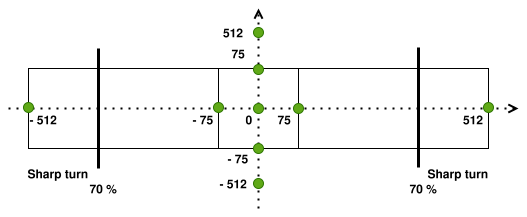
\includegraphics[width=0.85\textwidth]{images/diff_drive_logic.png}
    \caption{Differentialantrieb Logik}
    \label{fig:diff_drive_logic}
\end{figure}

Im Zentrum der Abbildung~\ref{fig:diff_drive_logic} befindet sich die Nullposition. Der Grund dafür wird im Abschnitt \ref{sec:diff_drive_integration} erläutert. Die beiden Kanäle im Bereich $|75|$ in X- bzw. Y-Richtung sind die Hysteresebereiche für die Geschwindigkeit bzw. die Drehung im Stand. Die äußeren Bereiche sind für das Fahren mit Lenkung relevant. Die 70 \% Markierungen symbolisieren dabei die Abgrenzung zwischen sanfter und harter Lenkung.

\subsection{Testing} \label{sec:diff_drive_tests}

Wie beim Testing des Low-Level Treibers, wurde der Code auch hier größtenteils KI-generiert. In der Summe gab es zwei Testszenarien:

\begin{itemize}
    \item Logik-Test auf Holzkonstruktion
    \item Logik-Test auf Laborboden
\end{itemize}

Im ersten Fall fielen gleich zu Beginn kleinere Fehler, wie beispielsweise das fehlerhafte Freigeben von Ressourcen, auf. Diese konnten umgehend behoben werden. Trotz der Anpassungen war ein größeres Problem ersichtlich: Die rechte Antriebsseite funktionierte nicht. Der linke Antriebsstrang lief zwar mit der korrekten Geschwindigkeit, dafür passten die Richtungswechsel nicht. \newline

Für Debuggung-Zwecke bietet das verwendete Framework ESP-IDF einen Loggingmechanismus an, der es ermöglicht, den Status von Variablen in Form von Konsolenausgaben nachzuvollziehen. Dafür ist es notwendig, dass der ESP32 über die USB-Schnittstelle mit dem Rechner verbunden ist. \newline

Folgendes Verhalten wurde festgestellt: Die Werte wurden korrekt berechnet, die Queue jedoch nicht richtig abgearbeitet. Das Problem lag bei der Initialisierung der Queue, welche Steuerbefehle entgegennimmt. Die API erlaubt es, Pointer auf Structs oder die komplette Größe des Structs als Queuewerte festzulegen. Im Code wurde beim Laden der Werte aus der Queue das komplette Struct angegeben, beim Laden in die Queue hingegen nur ein Pointer. Aufgrund der Pointergröße konnten nur die ersten 8-Byte richtige Werte enthalten, der Rest enthielt Zufallswerte. Durch Padding/Aligning des Compilers wurde die erste Variable (Speed links, float, 4 Byte) offensichtlich auf 8 Byte skaliert. Dadurch kam es zu dem undefinierten Verhalten, dass nur die linke Seite eine Drehzahl hatte. Die Richtung wurde aus einem Standardwert übernommen. Bei der rechten Seite traf man die Annahme, dass ein Zufallswert aus dem Speicher genommen wurde. Mit großer Wahrscheinlichkeit war dieser außerhalb des Bereichs, weshalb 0 (keine Drehzahl) angenommen wurde. Nach Anpassung des Übergabeparameters liefen beide Motoren mit der gewünschten Geschwindigkeit und die Richtungen entsprechend korrekt gewechselt. \newline

Im zweiten Fall wurde das Fahrzeug auf den Boden des Labors gestellt. Nach einem Timeout von 10 Sekunden sollte das Fahrzeug eine spezifizierte Routine durchlaufen, bei der das Drehverhalten im Stand, Beschleunigen bzw. Abbremsen und gegensätzliches Lenken getestet wurde. Die Beschleunigungstests verliefen durchwegs positiv. Tests, welche hingegen mit einer Drehung des Fahrzeugs bzw. Lenkung in Verbindung standen, wurden nicht erfolgreich abgeschlossen. Erste Versuche, die Ursache zu finden, ließen darauf schließen, dass die Motoren nicht ausreichend Leistung haben, um das Fahrzeug zu drehen. Nach eingehenden Untersuchungen - auch in Verbindung mit dem Betreuer - im Labor wurde festgestellt, dass die zuvor aufgelöteten Widerstände, die den Strom bei 6V Betriebsspannung begrenzen sollten, zu hoch dimensioniert waren. Selbst beim Anlegen einer höheren Spannung von 12V war es nicht möglich, das Fahrzeug zu drehen. Nach Entfernen der Widerstände und Anlegen von 12V Betriebsspannung konnte das Fahrzeug wie gewünscht drehen. \newline

\section{MQTT-Anbindung (Specht)}

Für den Semi-automatischen Modus ist es von zentraler Bedeutung, dass das Fahrzeug Befehle für die Geschützsteuerung empfangen kann. In Abstimmung mit dem Kollegen Jürgens wurde beschlossen, die Kommunikation zwischen KI-Komponente und Fahrzeug über MQTT umzusetzen. MQTT ist ein leichtgewichtiges Publish-Subscribe-Protokoll, das auch in Industrielösungen zum Einsatz kommt. Im ISO/OSI Referenzmodell entspricht es der Anwendungsschicht. In diesem Fall übernimmt der ESP32 die Rolle des Clients, der über einen zuvor festgelegten Topic Nachrichten empfängt. Die Vehicle-Control wurde deshalb so erweitert, dass sie auf den Topic lauscht. Demnach empfängt und verarbeitet die Vehicle-Control Nachrichten, die vom Zentralrechner, auf dem die KI-Komponente und der MQTT-Broker laufen, gesendet werden. \newline

\subsection{WiFi-Stack}

Der ESP32 bietet zwei Möglichkeiten, um eine Verbindung zu einem WLAN-Netzwerk herzustellen. Methode 1 nutzt die Hilfefunktion \textit{example\_connect}. Diese arbeitet beim Verbindungsaufbau nach dem Busy-Waiting-Prinzip, denn sie blockt so lange, bis eine Verbindung zum Netzwerk besteht und eine IP-Adresse zugewiesen wurde. Um die Verwendung der Funktion einfach zu gestalten, werden mögliche Fehlerfälle wie beispielsweise ein Timeout nicht ordentlich behandelt. Die Funktion ist somit nur begrenzt einsetzbar und für den produktiven Einsatz nicht geeignet. \newline

Ein weiterer Nachteil dieser Variante ist, dass das Setzen der Credentials (SSID und Passwort) normalerweise über die Konsole mittels \textit{idf.py menuconfig} erfolgt. Beim Testing fiel auf, dass dies auf dem im Projekt zum Einsatz kommenden ESP32 nicht funktioniert. \newline

Die zweite Methode nutzt die WiFi-API des ESP-IDF. Trotz erhöhter Komplexität bietet dieser Weg eine bessere Fehlerbehandlung und im Allgemeinen ein flexibleres Interface. Aufgrund dessen wurde sich für die zweite Methode entschieden. \newline

Aus dem Developer Portal von Espressif (cite) konnte eine Beispielimplementierung entnommen werden, die die grundlegende Funktionalität des Verbindungsaufbaus demonstriert. Diese wurde als Grundlage für die Implementierung der WiFi-Komponente verwendet. Trotz diverser Möglichkeiten, den WiFi-Stack noch zu optimieren, war die Idee diesen dennoch einfach zu halten. Hauptgrund für diese Entscheidung war, dass der WiFi-Stack und der damit verbundene MQTT-Stack zusätzliche Speicherresourcen benötigen, obwohl der Speicher aufgrund der Vielzahl an implementierten Komponenten bereits begrenzt ist. \newline

\subsection{MQTT-Stack}

Bevor mit der Programmierung begonnen werden konnte war es notwendig, sich mit der API des MQTT-Stacks auseinanderzusetzen. Abhilfe schaffte hierbei die Dokumentation des ESP-IDF (cite). Das Framework bietet neben TCP auch eine Reihe verschlüsselter Übertragungswege, wie beispielsweise SSL. Wegen der damit verbundenen erhöhten Komplexität und Einarbeitungszeit wurde sich aber in Absprache mit dem Kollegen Jürgens auf eine MQTT-Kommunikation mittels TCP geeinigt. Neben den Netzwerkeigenschaften und den API-Details enthält die Dokumentation auch Referenzen zu Beispielen in deren Github-Repository. So konnte die grundlegende Funktionalität anhand des Beispielscodes zügig erstellt werden. Das Programm stellt jedoch nur eine einfache Implementierung dar, die zur Orientierung dienen soll und für den Einsatz in größeren Projekten nicht geeignet ist. Deshalb waren weitere Anpassungen notwendig. Dabei wurde auf eine Kombination aus KI-generiertem Code, Beispielcode und eigener Implementierung zurückgegriffen. Die eigene Implementierung stützt sich dabei auf die Erkenntnisse aus der Analyse der Dokumentation. Darüber hinaus wurde großer Wert auf Konformität mit den bereits implementierten Komponenten gelegt. Dies betrifft insbesondere das Abfragen der Geschütz- und Feuersteuerung, das ebenfalls über Queues realisiert wird. \newline

Für die Verarbeitung der erhaltenen Nachrichten ist das Format der Daten von zentraler Bedeutung. Die Nachrichten werden im JSON-Format gesendet. Dies bietet einen einfachen Weg, um strukturierte Daten mit einem geringen Overhead zu übertragen. Die Nachrichten weisen dabei folgende Struktur auf:

\begin{lstlisting}
{
  "platform_x_angle": -45,
  "platform_y_angle": 80,
  "fire_command": true
}
\end{lstlisting}

Beide Winkel sind in der Einheit Grad angegeben. Der X-Winkel beschreibt die horizontale Ausrichtung des Geschützes im Bereich -90 bis +90 Grad, wobei -90 Grad nach links und +90 Grad nach rechts zeigt. Die Grad-Werte für den Y-Winkel bzw. die vertikale Orientierung liegen im Bereich 0 bis 80 Grad, wobei 48 Grad der Nullposition entspricht. Die Werte sind der Platform-Control entnommen und wurden vom Kollegen Becker entsprechend getestet. \newline

Das Kommando \textit{fire\_command} ist ein boolescher Wert, der angibt, ob das Geschütz feuern soll oder nicht. Prinzipiell ist dieser Wert im semi-automatischen Modus nicht relevant und somit immer \textit{false}, da der Feuerbefehl nur manuell ausgelöst werden kann. Um zukünftig eine automatische Feuersteuerung zu ermöglichen, wurde dieser Wert dennoch in die Nachrichtenstruktur aufgenommen. \newline

Die Nachrichten werden über den Topic \textit{vehicle/control} gesendet. Da im Projekt MQTT über TCP implementiert wrude, ist es potentiell möglich, dass von anderen Netzwerkteilnehmern Nachrichten an den Topic gesendet werden. Dies wurde jedoch nicht weiter berücksichtigt, da das Fahrzeug in einem dedizierten Netzwerk betrieben wird. \newline

\subsection{Testing}

Erste Tests der MQTT-Komponente konnten ohne Fahrzeug durchgeführt werden. Dazu wurde \textit{mosquitto} als MQTT-Broker auf dem Rechner installiert. Mit Hilfe des Tools \textit{mosquitto\_pub} können Nachrichten an den Topic gesendet werden. Mittels der bereits unter Abschnitt~\ref{sec:diff_drive_tests} beschriebenen Logging-Funktionalität des ESP-IDF konnte die korrekte Verarbeitung der Nachrichten mit Hilfe von Konsolenausgaben überprüft werden. Die Nachrichten wurden dabei korrekt empfangen.

\section{Integration/Fahrzeugsteuerung (Becker, Specht) \label{sec:esp32_integration}}

Die Fahrzeugsteuerung ist eine Abstraktionsebene, die als zentrale Anlaufstelle für Befehle vom Controller dient. Darin ist der Haupttask implementiert, der die Steuerbefehle entgegennimmt und an die entsprechenden Queues weiterleitet. Diese Queues werden dann von den Tasks der jeweiligen Komponenten abgearbeitet. Neben der Geschütz- und der Feuersteuerung ist auch die Ansteuerung der Differentialantrieb Logik eine der zentralen Komponenten. Darüber hinaus ist die Fahrzeugsteuerung auch das Modul, das letztendlich in der Main-Methode mithilfe diverser komponenten-spezifischer Strukturen initialisiert wird. \newline

\subsection{Regelschleife (Becker)}

Die Grundlage der Fahrzeugsteuerung bildet eine Regelschleife, welche synchron zur Update-Frequenz des DualShock4-Treibers mit 60 Hz ausgeführt wird. 
Zunächst wird in dieser Schleife gewartet, bis eine Verbindung zum Controller hergestellt wurde.
Im Anschluss daran wird der aktuelle Status des Controllers aus der entsprechenden Queue abgerufen (vgl. Abbildung \ref{fig:ds4_driver}).

Abhängig vom aktuellen Modus, also dem Zustand, in dem sich das Fahrzeug befindet, werden mit diesen Daten verschiedene Berechnungen durchgeführt. 
Das Fahrzeug verfügt über zwei Modi:

\begin{itemize}
    \item Im \textbf{manuellen Modus} erfolgt die Steuerung des Fahrzeugs, der Plattform sowie die Schussabgabe manuell über den DualShock4-Controller.
    \item Im \textbf{semi-automatischer Modus} wird die Steuerung der Plattform durch ein KI-Modell übernommen.
\end{itemize}

Der aktuelle Modus ist anhand der Lichtleiste des Controllers erkennbar:
Im manuellen Modus leuchtet die Lichtleiste in einem hellen Grün, während sie im semi-automatischen Modus in einem orangen Farbton leuchtet.
Der Modus kann durch gleichzeitiges Halten der oberen Pfeiltaste und der Kreuztaste für 1.5 Sekunden gewechselt werden, beim Moduswechsel vibriert der Controller für einen kurzen Moment.

\subsection{Plattformsteuerung \& Schussabgabe (Becker)} \label{sec:platform_integration}

Die Plattform wird im manuellen Modus anhand der Eingabe des Joysticks gesteuert, wobei zuerst die digitalisierten Werte des analogen Controller-Sticks in Winkel umgerechnet werden müssen.
Dafür werden folgende Schritte ausgeführt:

\begin{enumerate}
    \item \textbf{Deadzone-Filter} \newline
    Um kleine Bewegungen des Joysticks, die durch Stick-Drift entstehen, zu ignorieren, wird ein Deadzone-Filter angewendet.
    Wenn der Wert des Controller-Sticks kleiner als ein bestimmter Schwellenwert ist, wird der Wert auf null gesetzt, um ungewollte Eingaben zu vermeiden.
    \[
    \text{if} \left( |\text{stick}| < \text{deadzone} \right) \text{ then stick} = 0
    \]

    \item \textbf{Normalisierung} \newline
    Die vorliegenden Digitalwerte des Sticks werden nun vom Intervall ]-512, 512[ auf das Interval von ]-1, 1[ normalisiert.
    \[
    \text{normalized\_stick} = \frac{\text{stick}}{512}
    \]

    \item \textbf{Low-Pass-Filter zur Glättung der Eingabe} \newline
    Ein Low-Pass-Filter wird verwendet, um schnelle Schwankungen zu glätten und sanfte Bewegungen zu erzeugen. 
    Dieser wurde hinzugefügt, da es bei schneller Drehung durch heftiges Bewegen des Sticks häufig zu zitterigen Drehbewegungen kam.
    Der Filter berechnet einen geglätteten Wert basierend auf der aktuellen Eingabe sowie dem vorherigen Wert, wodurch schnelle Änderungen abgeflacht werden.
    \[
    \text{filtered\_stick} = \alpha \cdot \text{normalized\_stick} + (1 - \alpha) \cdot \text{filtered\_stick\_previous}
    \]

    Da \( \alpha = 0.2 \) beträgt, fließt die aktuelle Eingabe lediglich zu 20 Prozent in die Berechnung ein, während der vorherige Wert zu 80 Prozent berücksichtigt wird. 
    Dieser Wert wurde manuell gewählt, da hier zitterige Drehungen am besten verhindert werden.

    \item \textbf{Berechnung der Geschwindigkeit} \newline
    Die Geschwindigkeit der Plattform wird durch die gefilterte Eingabe sowie den maximalen Drehwinkel pro Sekunde berechnet. 
    So wird sichergestellt, dass die Plattform lediglich mit einer Geschwindigkeit rotiert, die von den Servos verarbeitet werden kann. 
    Der Wert wurde anhand des Datenblatts \cite{esp_platform_servo} festgelegt und anschließend an beiden Plattformachsen reduziert, um eine übermäßige Empfindlichkeit gegenüber Controller-Eingaben zu vermeiden.
    \[
    \text{speed} = \text{filtered\_stick} \cdot \text{max\_deg\_per\_sec}
    \]

    \item \textbf{Berechnung des neuen Winkels} \newline
    Schließlich wird der Winkel der Plattform auf Basis der berechneten Geschwindigkeit und der Zeitdifferenz ($dt$, der Abstand zwischen den Regelzyklen) angepasst. 
    \[
    \text{platform\_angle} = \text{platform\_angle} \pm (\text{speed} \cdot \text{dt})
    \]
    Ob Addition oder Subtraktionverwendet wird, basiert hierbei auf der Verbaurichtung des Servomotors.
\end{enumerate}

Durch diese Berechnungen lässt sich die Plattform nun über die vertikale Achse des rechten Sticks des DualShock4-Controllers drehen und über die horizontale Achse neigen. 
Bedauerlicherweise führen die Vibrationen des Geschützaufbaus, insbesondere bei längerer und schnellerer Drehung, weiterhin zu ruckartigen Bewegungen der Motoren. 
Es konnte beobachtet werden, dass sich das Verhalten durch den Einsatz eines Low-Pass-Filters marginal verbessert hat. Aufgrund von Zeitmangel konnten keine weiteren Lösungsansätze mehr in Betracht gezogen werden. 
Ein möglicher Ansatz wäre beispielsweise der Wechsel der Servomotoren zu digitalen Motoren, die ein genaueres Feedback liefern, oder der Einbau einer PID-Regelung.

Zusätzlich wird, sobald der Nutzer die Enden der Drehwinkel erreicht hat, haptisches Feedback in Form von Vibration des Controllers an den Nutzer weitergegeben. 
Durch das Halten der Kreistaste ist es im manuellen Modus ebenfalls möglich, sich zurück auf die Nullposition beider Achsen zu bewegen.

Die Schussabgabe erfolgt über den rechten unteren Trigger des Controllers, analog zur Steuerung in bekannten Shootern. 
Da der Treiber die Position des Triggers als 10-Bit-Wert liefert, wurde ein Threshold-Wert von 800 gewählt, um wirklich nur gewollten Druck zu registrieren und nicht versehentlich Schüsse abzufeuern.

\subsection{Differentialantrieb (Specht)} \label{sec:diff_drive_integration}

Die Integration in die bestehende Code-Basis war relativ unkompliziert, da das Abgreifen der Steuerbefehle über den PS4-Treiber einfach handzuhaben ist. Ein Struct enthält alle notwendigen Stick- bzw. Button-Werte, die am Controller gedrückt werden. Problematisch war jedoch der Stick-Drift des linken Sticks, denn dadurch wurde der PS4-Treiber ständig mit Werten versorgt, was zu einer permanenten Anpassung der Geschwindigkeit führte. Die ersten Befehle konnten teilweise noch übermittelt werden, jedoch lief nach kurzer Zeit die Queue über und es kam zu einem Absturz des Programms. \newline

Die Lösung des Problems bestand darin, den Stick-Drift einzudämmen. Daraufhin wurde durch Ausprobieren am Fahrzeug ein Wert ermittelt, ab dem ein neuer Befehl interpretiert werden sollte. Dieser Wert wurde in der Fahrzeugsteuerung als Deadzone definiert. Wenn der linke Stick des Controllers innerhalb dieser Deadzone bewegt wird, wird die Geschwindigkeit des Fahrzeugs nicht angepasst. Dadurch wird verhindert, dass die Queue überläuft und das Programm abstürzt. \newline

Allerdings wurde infolgedessen festgestellt, dass die Queue im Stand überläuft, wenn der linke Stick nicht bewegt wird. Das Problem war, dass die bis dato verwendete Logik die Nullposition als normalen Fahrbefehl interpretierte und somit ständig Werte sendete. \newline

Deshalb wurde, wie im Zentrum der Abbildung~\ref{fig:diff_drive_logic} zu sehen, eine Nullposition definiert. Diese wird beim Auftreten, sprich Nicht-Bewegen des linken Sticks, detektiert. Daraufhin wird ein Stop eingeleitet. Sobald dieser abgearbeitet wurde wird ein Flag gesetzt, das anzeigt, dass die Nullposition bereits abgearbeitet wurde. Somit wird verhindert, dass das Stoppen unnötig wiederholt wird und die Queue überläuft. Sobald der linke Stick wieder bewegt wird, wird das Flag zurückgesetzt und die Geschwindigkeit des Fahrzeugs angepasst. \newline

\subsection{MQTT-Anbindung (Specht)}